\chapter{Opis projektnog zadatka}
		
<<<<<<< HEAD
		\textbf{\textit{dio 1. revizije}}\\
		
		\textit{Na osnovi projektnog zadatka detaljno opisati korisničke zahtjeve. Što jasnije opisati cilj projektnog zadatka, razraditi problematiku zadatka, dodati nove aspekte problema i potencijalnih rješenja. Očekuje se minimalno 3, a poželjno 4-5 stranica opisa.	Teme koje treba dodatno razraditi u ovom poglavlju su:}
		\begin{packed_item}
			\item \textit{potencijalna korist ovog projekta}
			\item \textit{postojeća slična rješenja (istražiti i ukratko opisati razlike u odnosu na zadani zadatak). Dodajte slike koja predočavaju slična rješenja.}
			\item \textit{skup korisnika koji bi mogao biti zainteresiran za ostvareno rješenje.}
			\item \textit{mogućnost prilagodbe rješenja }
			\item \textit{opseg projektnog zadatka}
			\item \textit{moguće nadogradnje projektnog zadatka}
		\end{packed_item}
		
=======
		
		\textit{"WebGym"} je web aplikacija namijenjena svim ljudima željnim organizacije 
		svog vježbanja u teretanama. Korisnicima aplikacije bit će moguće pregledavanje 
		dostupnih teretana, njihovih cijena, pregled trenera koji nude privatne ili grupne 
		treninge, pregled ponuda planova vježbanja i planova prehrane trenera kao i 
		mogućnost zadavanja vlastitih ciljeva te vođenje evidencije o njihovom ostvarivanju.
		Također ova web aplikacija omogućit će trenerima jednostavnije spajanje s klijentima,
		komunikaciju s teretanama te će im potencijalno proširiti tržište. Teretanama će pak 
		ovo omogućiti odlično mjesto za prezentaciju svoje ponude jer će ovo biti platforma 
		na kojoj će svi jednostavno moći pregledavati njihovu ponudu, te će onim teretanama 
		s najboljim omjerom cijene i kvalitete potencijalno povećati broj korisnika. 
		
		\vspace{5mm}
		
		Na internetu nismo uspjeli pronaći pandan našoj platformi niti platformu koja 
		nudi veći opseg od naše platforme, ali neka slična rješenja postoje te će u nastavku 
		biti detaljnije opisana. 
		
		Stranica \href{https://www.trainerize.me/}{Trainerize.me (https://www.trainerize.me/)} nudi platformu na kojoj je vrlo jednostavno moguće pronaći osobnog trenera, vidjeti 
		njegov opis te ga je moguće kontaktirati putem poruke. Trenere je moguće pretraživati po lokaciji, popularnosti, vrsti vježbanja koje nude te još mnogo toga. 
		Treneri također mogu nuditi online treninge kao i treninge u teretanama. Stranica 
		trenerima daje mjesto na kojem se oni mogu oglašavati te ih čini puno vidljivijima na 
		tržištu. Također im zbog mogućnosti online treninga znatno proširuje tržište. Stranica uz sve već navedeno nudi i mogućnost objavljivanja te čitanja članaka 
		vezanih uz treniranje.
		
		\begin{figure}[H]
			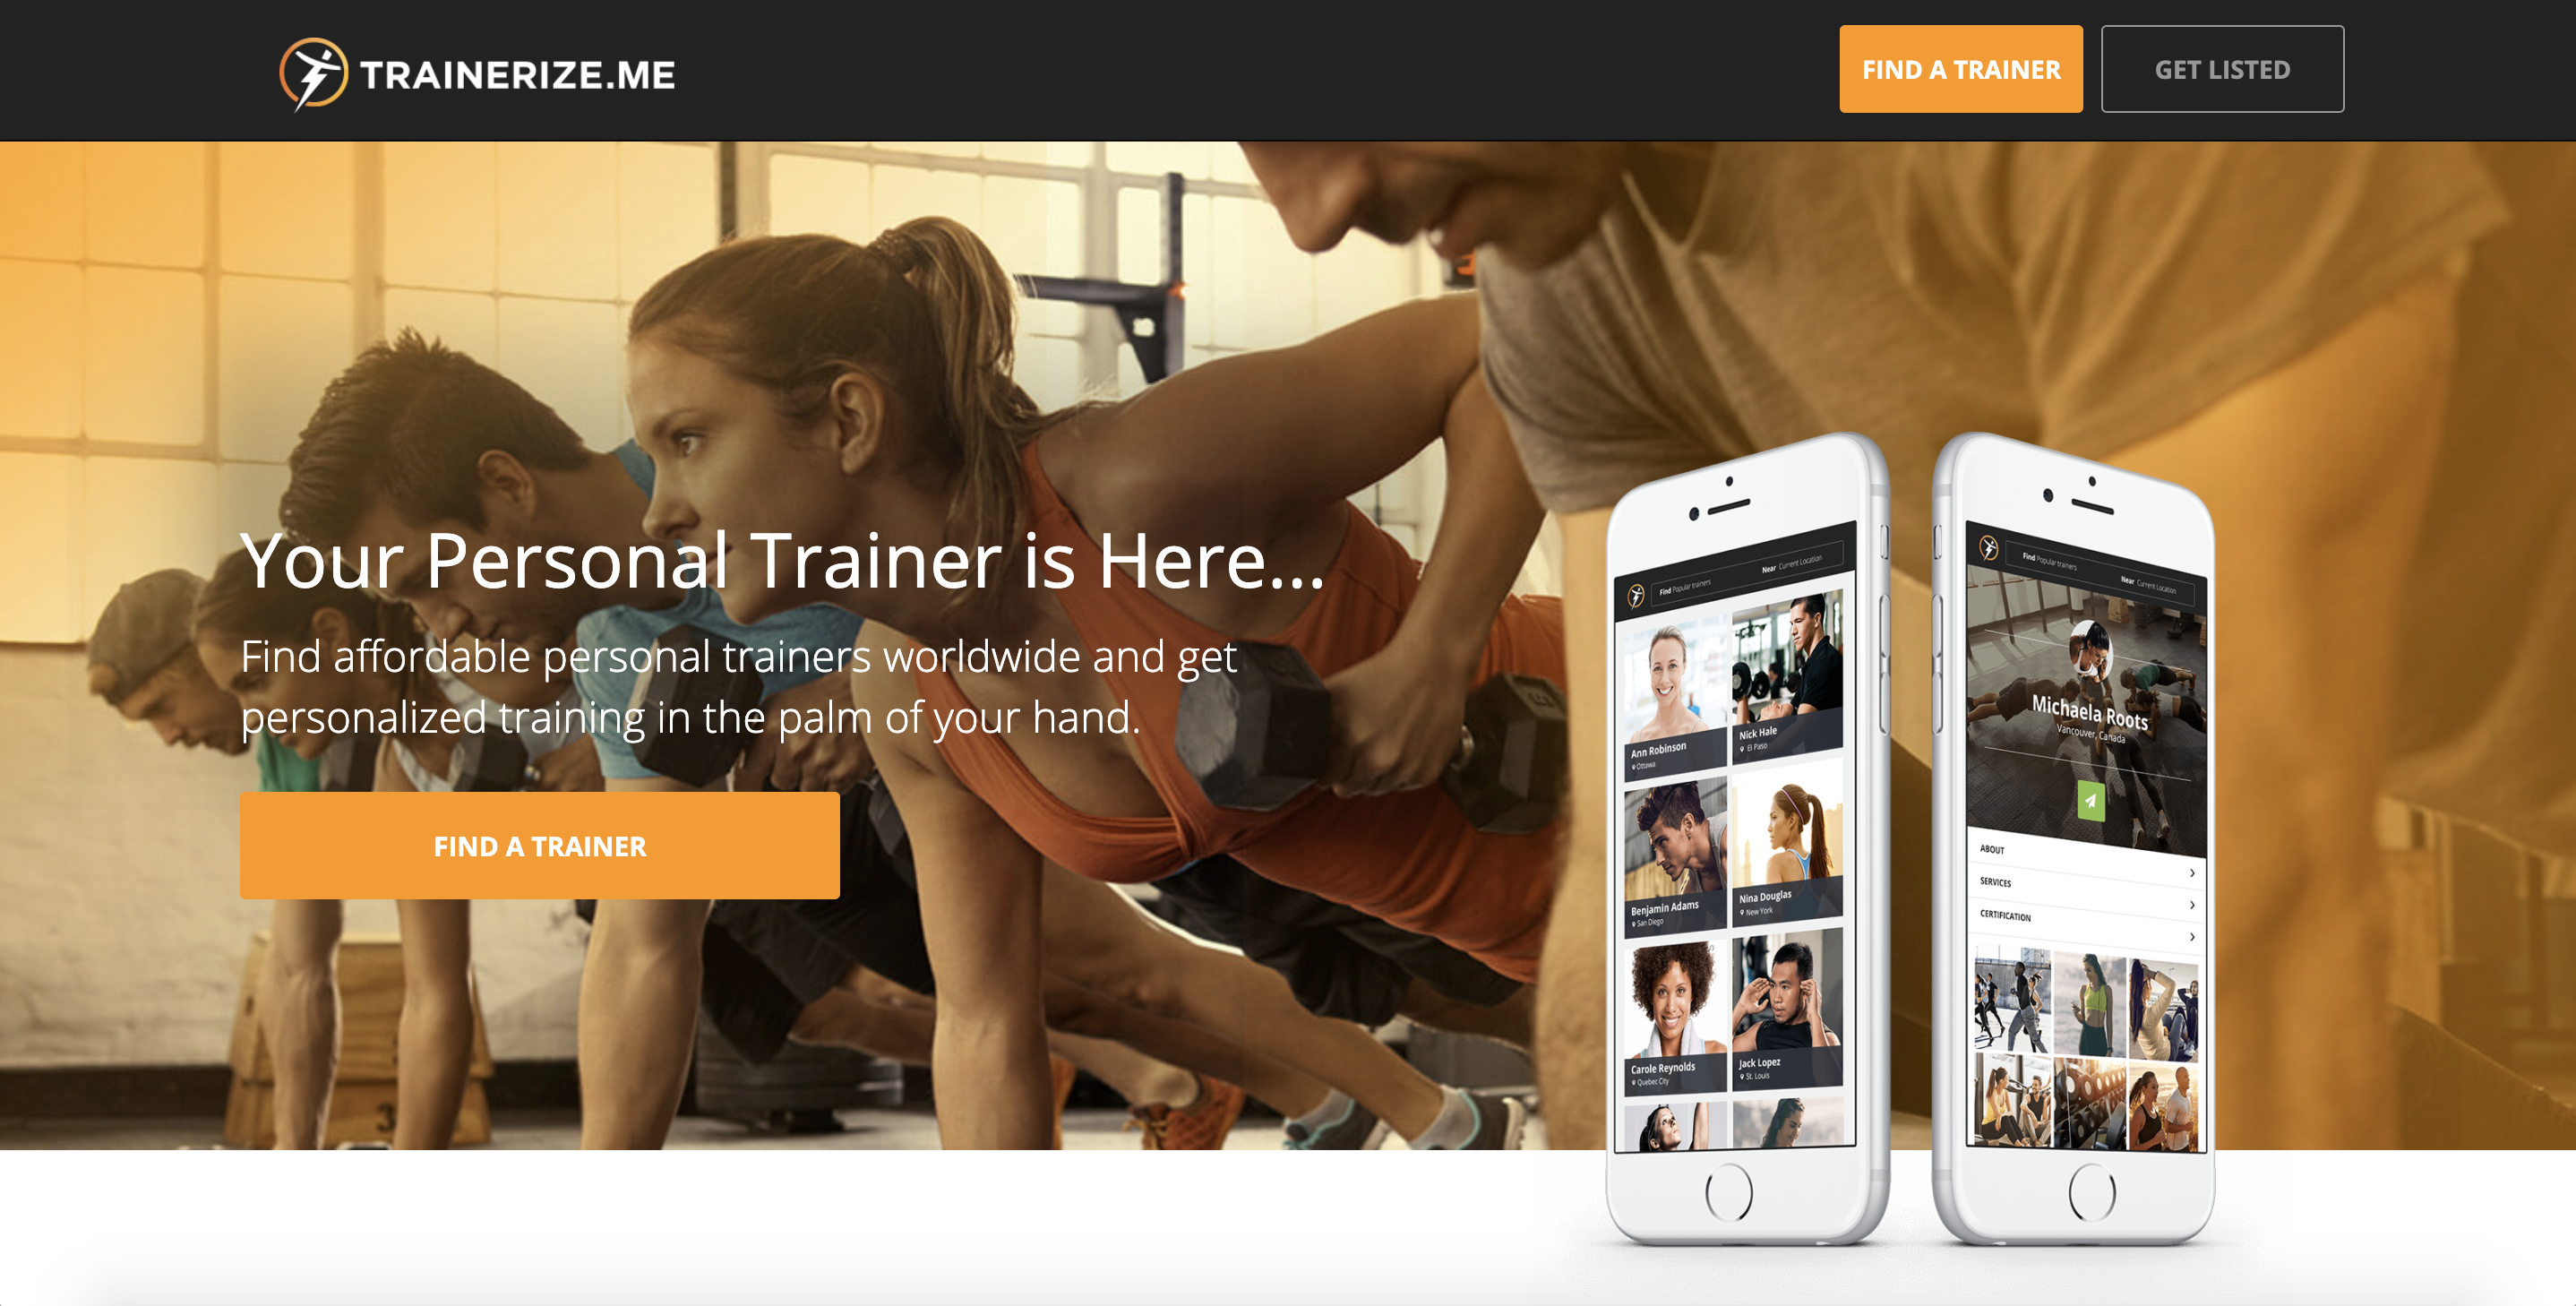
\includegraphics[scale=0.20]{slike/trainerizeme1.PNG} %veličina slike u odnosu na originalnu datoteku i pozicija slike
			\centering
			\caption{Početna stranica https://www.trainerize.me/}
			\label{fig:promjene}
		\end{figure}
	
		\begin{figure}[H]
			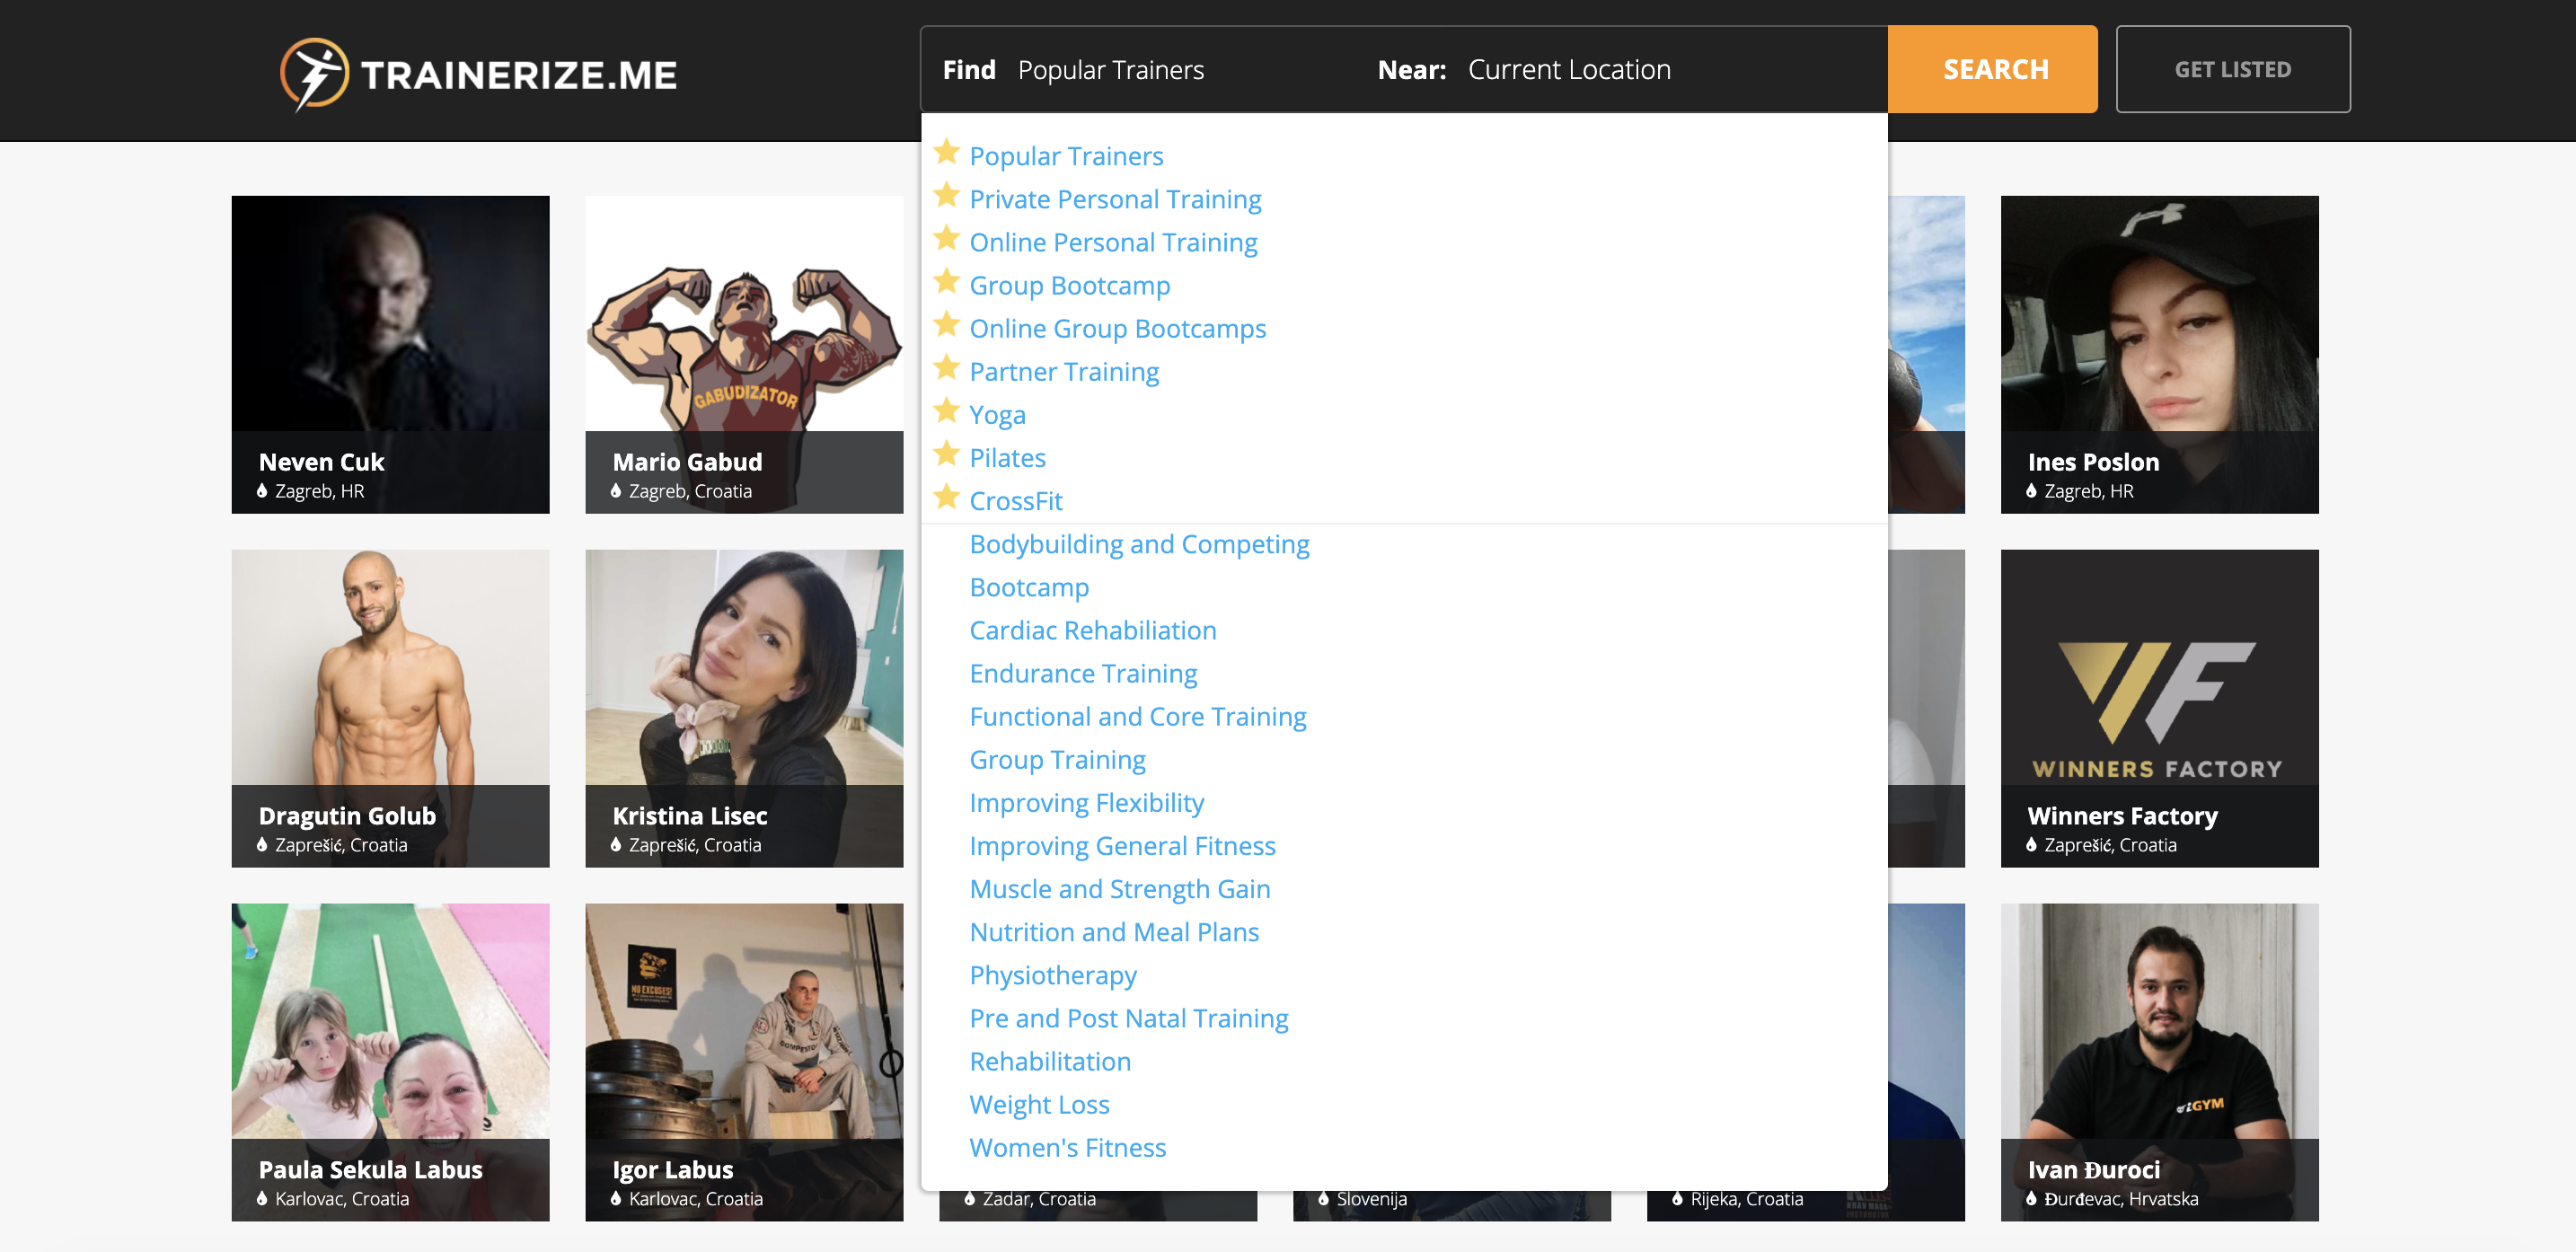
\includegraphics[scale=0.20]{slike/trainerizeme2.PNG} %veličina slike u odnosu na originalnu datoteku i pozicija slike
			\centering
			\caption{Pretraživanje trenera https://www.trainerize.me/}
			\label{fig:promjene}
		\end{figure}
	
		Stranica \href{https://ultimateperformance.com/}{Ultimate Performance (https://ultimateperformance.com/)} nudi gotove planove vježbanja za određene
		svrhe, kao što su gubljenje kilograma, dobivanje mišićne mase i slično, također 
		su programi podijeljeni po spolovima. Također je moguće dogovoriti konzultacije 
		s osobnim trenerima te naručivati personalizirane planove vježbanja.
		
		\begin{figure}[H]
			
\includegraphics[scale=0.20]{slike/ultimateperformance.PNG} %veličina slike u odnosu na originalnu datoteku i pozicija slike
			\centering
			\caption{Početna stranica https://ultimateperformance.com/}
			\label{fig:promjene}
		\end{figure}
		
		\vspace{5mm}
		
		Cilj ovog projekta je razviti programsku podršku za stvaranje web aplikacije
		\textit{"WebGym"} koja će svojim korisnicima uvelike olakšati administrativne 
		poslove vezane uz njihove odlaske u teretanu. Cilj platforme \textit{"WebGym"} 
		je poboljšavanje ukupnog doživljaja teretane, a namijenjena je neregistriranim 
		korisnicima, registriranim korisnicima, trenerima u teretani i voditeljima svake od 
		teretana (jedan voditelj može biti zadužen za više
		teretana i za svaku teretanu može biti zaduženo više voditelja). Za registraciju bilo kojeg od korisnika potrebno je unijeti
		ime, prezime, email adresu i osobne podatke bitne za trenere (visina, težina…) te je PayPal račun opcionalan. 
		
		Prilikom pokretanja sustava (odlaska na početnu stranicu) ukoliko korisnik nije trenutno prijavljen pokazuje se općenita početna stranica. Na toj početnoj stranici u gornjem desnom kutu nalaze se polja za unos korisničkog imena i lozinke te gumb za registraciju korisnika koji se do sada nisu registrirali. Na početnoj stranici se za neregistrirane korisnike nalazi popis najpopularnijih teretana, a svaka teretana u tom popisu ima prikazanu svoju profilnu sliku, ime i adresu teretane.
		
		Za kreiranje novog računa potrebni su sljedeći podaci:

		\begin{packed_item}
			\item Korisničko ime
			\item Ime
			\item Prezime
			\item Broj mobitela
			\item e-mail
		\end{packed_item}
	
		Također opcionalno se mogu unijeti i sljedeći podatci:
		
		\begin{packed_item}
			\item PayPal račun
			\item Visina
			\item Težina
		\end{packed_item}
	
		Pri izradi korisničkog računa moguće je odabrati jednu od tri opcije:
		
		\begin{packed_item}
			\item Korisnik teretana
			\item Voditelj teretane
			\item Trener
		\end{packed_item}
	
		Običan registrirani korisnik je osoba koja je izradila račun s namjerom pohađanja teretane radi vježbanja.
		Korisnik može pregledavati teretane, plaćati članarine u njima putem interneta, vidjeti u kojim sve teretanama
		može vježbati s već uplaćenim članarinama (jedan lanac teretana može imati više teretana i korisnik može
		plaćati članarinu u više teretana), također za svaku teretanu se vodi i datum isteka trenutne članarine. Korisnik
		može također trenerima plaćati planove prehrane ili vježbanja te privatne i grupne treninge. Korisnik uz sve
		ovo može imati i svoj plan vježbanja te na samoj stranici može voditi napredak u svom planu.
	
		Treneri su korisnici koji su pri izradi korisničkog računa kliknuli na opciju izrade trenerskog računa. Treneri na
		svojoj stranici mogu nuditi planove treninga i prehrane, kao i individualno ili grupno vježbanje, a sve ranije
		opcije mogu biti besplatne ili ih treneri mogu naplaćivati. Treneri mogu organizirati i grupno vježbanje u
		teretanama u kojima im je voditelj dao tu ovlast, odnosno stavio ih na popis trenera te teretane.
	
		
		Treneri i obični korisnici mogu pregledati sve izvršene transakcije u kojima su sudjelovali, a voditelji mogu
		vidjeti sve transakcije koje su se izvršile na aplikaciji u sklopu teretana koje vode.
		
		Administrator je korisnik koji je pri izradi svojeg korisničkog računa kliknuo na izradu administratorskog
		računa. Administrator ima sve voditeljske privilegije nad svim teretanama te može vidjeti sve izvršene
		transakcije. On može brisati i pregledavati i sve teretane i sve račune korisnika.
		
		Voditelj teretane je korisnik koji je izradio svoj korisnički račun i pri tome kliknuo da izrađuje voditeljski račun.
		Svaki voditelj može stvarati nove teretane u sustavu te on može davati dozvolu drugim voditeljima da vode
		neku od teretana za koje je on voditelj. Uloga voditelja je postavljanje teretane u sustav te promjene bitnih
		informacija o toj teretani (promjena lokacije, radnog vremena i sl.). Voditelj također može dodavati
		registrirane trenere u svoju teretanu, odnosno može im dopustiti rad u svojoj teretani te će se trener nakon
		toga pokazati na popisu trenera u toj teretani.
		
	
	
		\vspace{5mm}
		
		Mogućnosti nadogradnje ovog projektnog zadatka su mnogobrojne. Moguće je uvesti chat u kojem bi se trenerima i njihovim polaznicima treninga pružila mogućnost izravnog dopisivanja o planu vježbanja, potencijalnim novim ponudama i 
		još mnogo toga. Chat bi se također mogao koristiti između više voditelja iste teretane kako bi mogli koordinirati svoje akcije na platformi ili općenito veze uz poslovanje teretane. Također bi i komunikacija trenera i teretana uvođenjem ove 
		opcije bila uvelike olakšana te bi bila mnogo kvalitetnija. 
		
		Druga potencijalna mogućnost nadogradnje bi bila uvođene online dućana u kojemu 
		bi svaka teretana mogla svojim klijentima nuditi proizvode kao što su suplementi za 
		teretanu, opremu za treniranje i slično. Također bi se mogao uvesti jedinstveni 
		dućan na razini platforme u kojemu bi vlasnici platforme mogli nuditi proizvode ili bi 
		taj dućan mogao biti izveden kao mjesto na kojem dućani koji prodaju suplemente ili 
		opremu za treniranje mogu nuditi svoje proizvode. Ukoliko se dućan odluči izvesti na 
		drugi način u sustavu bi se trebala dodati mogućnost stvaranja dućana te njihovih 
		zaposlenika (to bi bilo izvedeno vrlo slično kao i za teretanu te za voditelje teretana).
		
		
	
		\vspace{5mm}
	
			
>>>>>>> devdoc
		\textit{Za pomoć pogledati reference navedene u poglavlju „Popis literature“, a po potrebi konzultirati sadržaj na internetu koji nudi dobre smjernice u tom pogledu.}
		\eject
		
		\section{Primjeri u \LaTeX u}
		
		\textit{Ovo potpoglavlje izbrisati.}\\

		U nastavku se nalaze različiti primjeri kako koristiti osnovne funkcionalnosti \LaTeX a koje su potrebne za izradu dokumentacije. Za dodatnu pomoć obratiti se asistentu na projektu ili potražiti upute na sljedećim web sjedištima:
		\begin{itemize}
			\item Upute za izradu diplomskog rada u \LaTeX u - \url{https://www.fer.unizg.hr/_download/repository/LaTeX-upute.pdf}
			\item \LaTeX\ projekt - \url{https://www.latex-project.org/help/}
			\item StackExchange za Tex - \url{https://tex.stackexchange.com/}\\
		
		\end{itemize} 	


		
		\noindent \underbar{podcrtani tekst}, \textbf{podebljani tekst}, 	\textit{nagnuti tekst}\\
		\noindent \normalsize primjer \large primjer \Large primjer \LARGE {primjer} \huge {primjer} \Huge primjer \normalsize
				
		\begin{packed_item}
			
			\item  primjer
			\item  primjer
			\item  primjer
			\item[] \begin{packed_enum}
				\item primjer
				\item[] \begin{packed_enum}
					\item[1.a] primjer
					\item[b] primjer
				\end{packed_enum}
				\item primjer
			\end{packed_enum}
			
		\end{packed_item}
		
		\noindent primjer url-a: \url{https://www.fer.unizg.hr/predmet/proinz/projekt}
		
		\noindent posebni znakovi: \# \$ \% \& \{ \} \_ 
		$|$ $<$ $>$ 
		\^{} 
		\~{} 
		$\backslash$ 
		
		\begin{longtabu} to \textwidth {|X[8, l]|X[8, l]|X[16, l]|} %definicija širine tablice, širine stupaca i poravnanje
			
			%definicija naslova tablice
			\hline \multicolumn{3}{|c|}{\textbf{naslov unutar tablice}}	 \\[3pt] \hline
			\endfirsthead
			
			%definicija naslova tablice prilikom prijeloma
			\hline \multicolumn{3}{|c|}{\textbf{naslov unutar tablice}}	 \\[3pt] \hline
			\endhead
			
			\hline 
			\endlastfoot
			
			\rowcolor{LightGreen}IDKorisnik & INT	&  	Lorem ipsum dolor sit amet, consectetur adipiscing elit, sed do eiusmod  	\\ \hline
			korisnickoIme	& VARCHAR &   	\\ \hline 
			email & VARCHAR &   \\ \hline 
			ime & VARCHAR	&  		\\ \hline 
			\cellcolor{LightBlue} primjer	& VARCHAR &   	\\ \hline 
			
		\end{longtabu}
		

		\begin{table}[H]
			
			\begin{longtabu} to \textwidth {|X[8, l]|X[8, l]|X[16, l]|} 
				
				\hline 
				\endfirsthead
				
				\hline 
				\endhead
				
				\hline 
				\endlastfoot
				
				\rowcolor{LightGreen}IDKorisnik & INT	&  	Lorem ipsum dolor sit amet, consectetur adipiscing elit, sed do eiusmod  	\\ \hline
				korisnickoIme	& VARCHAR &   	\\ \hline 
				email & VARCHAR &   \\ \hline 
				ime & VARCHAR	&  		\\ \hline 
				\cellcolor{LightBlue} primjer	& VARCHAR &   	\\ \hline 
				
				
			\end{longtabu}
	
			\caption{\label{tab:referencatablica} Naslov ispod tablice.}
		\end{table}
		
		
		%unos slike
		\begin{figure}[H]
			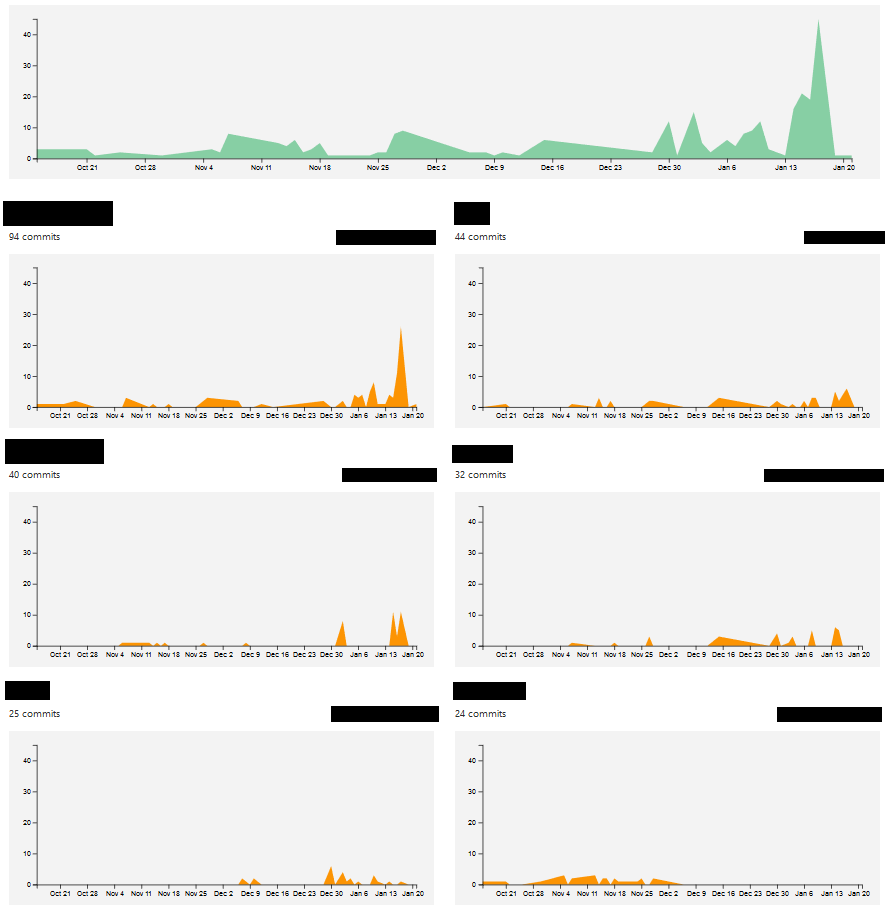
\includegraphics[scale=0.4]{slike/aktivnost.PNG} %veličina slike u odnosu na originalnu datoteku i pozicija slike
			\centering
			\caption{Primjer slike s potpisom}
			\label{fig:promjene}
		\end{figure}
		
		\begin{figure}[H]
			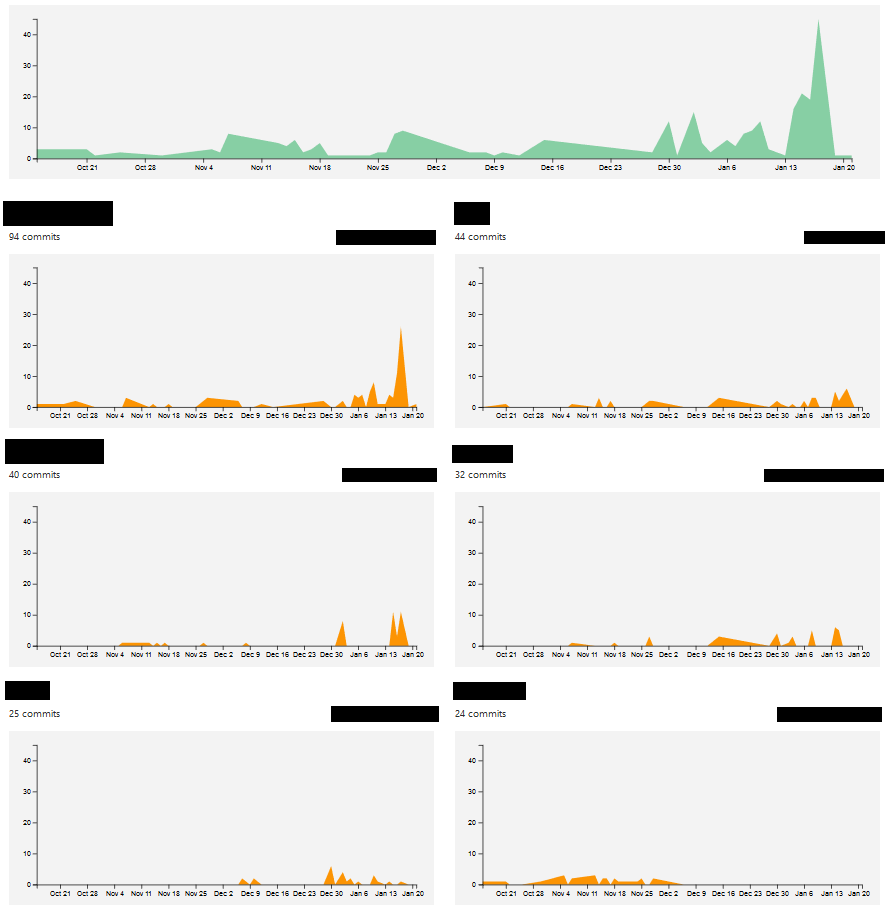
\includegraphics[width=.9\linewidth]{slike/aktivnost.PNG} %veličina u odnosu na širinu linije
			\caption{Primjer slike s potpisom 2}
			\label{fig:promjene2} %label mora biti drugaciji za svaku sliku
		\end{figure}
		
		Referenciranje slike \ref{fig:promjene2} u tekstu.
		
		\eject
		
	